\documentclass{article}
\usepackage[utf8]{inputenc}
\usepackage{graphicx}
\usepackage{geometry}
\usepackage{hyperref}
\hypersetup{
    colorlinks,
    citecolor=black,
    filecolor=black,
    linkcolor=black,
    urlcolor=black
}

 \geometry{
 a4paper,
 left=30mm,
 right=30mm,
 top=30mm,
 }

\graphicspath{ {Images/} }

%----------------------------------------------------------------------------------------
%	TITLE PAGE
%----------------------------------------------------------------------------------------

\newcommand*{\titleGP}{\begingroup
		\begin{figure}[t]
			\centering
			
\includegraphics[width=350px]{UP_Logo.PNG}
		\end{figure}
\centering 
\vspace*{\baselineskip}

\rule{\textwidth}{1.6pt}\vspace*{-\baselineskip}\vspace*{2pt}
\rule{\textwidth}{0.4pt}\\[\baselineskip]

{\LARGE NavUP\\ [0.3\baselineskip] Longsword Testing Report } \\ [0.2\baselineskip]
\rule{\textwidth}{0.4pt}\vspace*{-\baselineskip}\vspace{3.2pt}
\rule{\textwidth}{1.6pt}\\[\baselineskip] %

% \scshape %
% A concise specification on the functional requirements  \\
% and use cases of NavUP \\[\baselineskip]

% \vspace*{2\baselineskip}

Compiled By \\[\baselineskip]
{\Large Lucian Sargeant - u15225560 \\ Ritesh Doolabh - u15075754 \\ Peter Boxall -  u14056136 \\ Claude Greeff - u13153740\\ Harris Leshaba - u15312144 \\ Hristian Vitrychenko - u15006442\par}

\bigskip
\bigskip

 	GitHub Repository:  
 	\href{https://github.com/Chris19951225/COS-301-Longsword-Data-Streaming}{COS 301 Team Longsword Data GitHub Repository(Phase 4)}




 

\vfill


{\scshape 2017} \\[0.3\baselineskip]
{\large TEAM LONGSWORD (DATA)}\par

\endgroup}

\begin{document}

\titleGP
\newpage
\tableofcontents

\newpage
\section{Introduction}
\begin{flushleft}
For this phase we will be testing the Data module of the BroadSword Team. We have split the testing phase according to Functional Requirements, Non-Functional Requirements and Use Cases. 
\end{flushleft}

\begin{flushleft}
Their code was primarily coded in Python and used a NSQ message processing system.
We will be testing the various cases and giving a brief description of how we tested followed by an explanation of the mark that was given to them.
\end{flushleft}


\section{Service Contracts}

\subsection{Retrieving and passing device MAC address.}
\begin{flushleft}MARK: 10\end{flushleft}
The access module sends a location request to the data module via the NSQ server,the access module has to subscribes to a topic.The main entry point of the system, query\_resolver.py, sends the mac address to the aruba server in a query to get the location of the device.
In query\_resolver.py, the handler function receives a request, it then passes the mac address to the searcher function-which will create a query to get the location for the device.
\begin{flushleft}This functional requirement was fulfilled by the Broadsword team.\end{flushleft}
\begin{figure}[ht]
  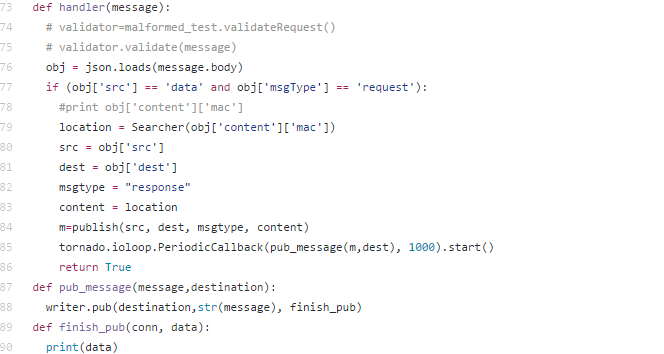
\includegraphics[width=350px]{Handler.jpg}
  \caption{Handler function.}
  \label{fig:Handler function}
\end{figure}

\subsection{Logging in and maintaining a session with Aruba ALE.}

\subsection{Processing the request and retrieving location.}
\begin{flushleft}MARK: 5\end{flushleft}
In the Broadword python file location\_lookup.py, they attempt to connect to Aruba by importing and using aruba\_wrapper.py. 
They then attempt to send a request to Aruba with a mac address, expecting a raw JSON object in return. They then return 
sta\_location\_x, sta\location\_y, building\_id and floor\_id from the raw JSON object. The reason they only got half of the marks
is because they do not actually get an existing location, rather resorting to hard coded, mock JSON that they themselves provide 
from a file called mock_location_json. This was further proven to be the case when testing the program returned a JSON object despite the lack of LAN or any type of connection to Aruba whatsoever. 
\begin{flushleft}This functional requirement was not fully fulfilled by the Broadsword team.\end{flushleft}

\subsection{Returning a location to the source of the request.}


\section{Non-Functional Requirements}

\subsection{Level of concurrency of the task.}

\subsection{Performance of the request processing (time taken to receive a response).}

\subsection{Maintainability and modularity of the code and repository.}

\subsection{Integrability and ease of transfer into a final system.}


\section{Use Cases}

\subsection{Upstream communication.}

\subsection{Downstream communication.}

\end{document}
